\chapter{Experiments and Methods}\label{chapter:experiments}
In the course of the thesis, several domain adaptation approaches were applied on two datasets to investigate the performance gains achieved by domain adaptation modules in PHM systems. In the following, a synthetically generated dummy dataset and a dataset recorded on an industrial milling machine are presented. Besides that, the domain shift in the real-world dataset and the corresponding classification task is explained. Lastly, the final model and the corresponding training strategy are explained.

\section{Dummy Dataset}
As a first evaluation, different domain adaptation approaches for PHM applications were evaluated on a synthetically generated dummy dataset. Such a dataset is structured equally and shows similar patterns as the corresponding real-world dataset. The complexity of the data and therefore the task itself can be tuned arbitrarily. A dummy dataset can help to understand underlying mechanisms and processes when applying a new and unknown approach for a given task. Besides that, it serves as a prior evaluation of the approach's applicability for the corresponding real-world task. In this work, a simple dummy dataset, suffering from a domain shift, was established to evaluate, how MMD-losses can optimize neural networks to extract more domain invariant features. Since one has to deal with irregularities, outliers and noise in real-world data, it is helpful to evaluate the MMD-loss on a dataset, which is not disturbed by these effects. Similarly to PHM applications, the dummy dataset contains one-dimensional time sequences. In the dummy example, the time sequences consists of 1000 data points, which are sampled from a cosine curve. In order to simulate the classification problem with two classes and two domains the data points are sampled from four cosine curves with characteristic amplitudes and frequencies. By adjusting the amplitude and frequency, the domain adaptation problem can be configured more or less difficult. The sampling process must include a certain randomness to allow variations in sequences of the same class and domain. For every sampling step, the characteristic amplitude and frequency of the cosine curve is perturbed. This changes the underlying characteristic of each sequence. Besides that, noise is added to each of the 1000 data points. This is necessary to generate a periodic signal which is close to a noisy real-world vibration signal. Exemplary, fig. \ref{fig:samples_domain_class_dummy} shows four sequence for each class and domain. 

\begin{figure}[H]
  \centering
  \includegraphics[width=.45\textwidth]{samples_domain_class_dummy/Source_Domain_Class_0_obs_0.pdf}
  \hspace{.3cm}
  \includegraphics[width=.45\textwidth]{samples_domain_class_dummy/Source_Domain_Class_1_obs_0.pdf}

  \vspace{.3cm}

  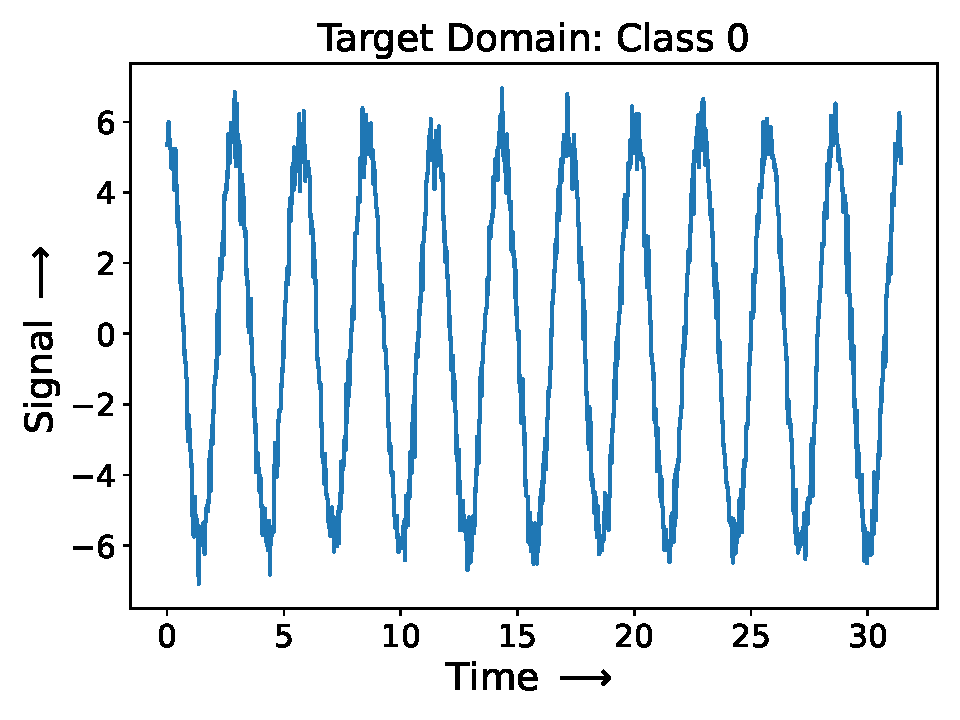
\includegraphics[width=.45\textwidth]{samples_domain_class_dummy/Target_Domain_Class_0_obs_0.pdf}
  \hspace{.3cm}
  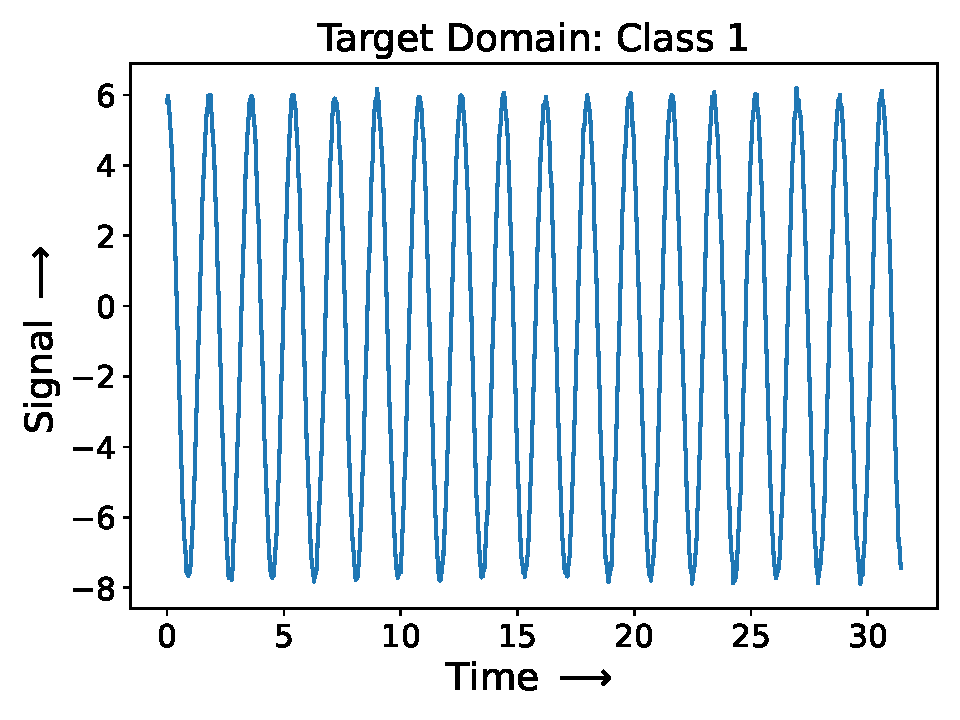
\includegraphics[width=.45\textwidth]{samples_domain_class_dummy/Target_Domain_Class_1_obs_0.pdf}

  \caption{Data window samples for each domain and class}
  \label{fig:samples_domain_class_dummy}
\end{figure}

In fig. \ref{fig:samples_domain_class_dummy_influence_noise} one can see how the perturbation and noise applied during the sampling process changes the data sequences belonging to the same class and domain. 

\begin{figure}[H]
  \centering
  \includegraphics[width=.45\textwidth]{samples_domain_class_dummy_influence_noise/Source_Domain_Class_0_obs_0.pdf}
  \hspace{.3cm}
  \includegraphics[width=.45\textwidth]{samples_domain_class_dummy_influence_noise/Source_Domain_Class_1_obs_0.pdf}

  \vspace{.3cm}

  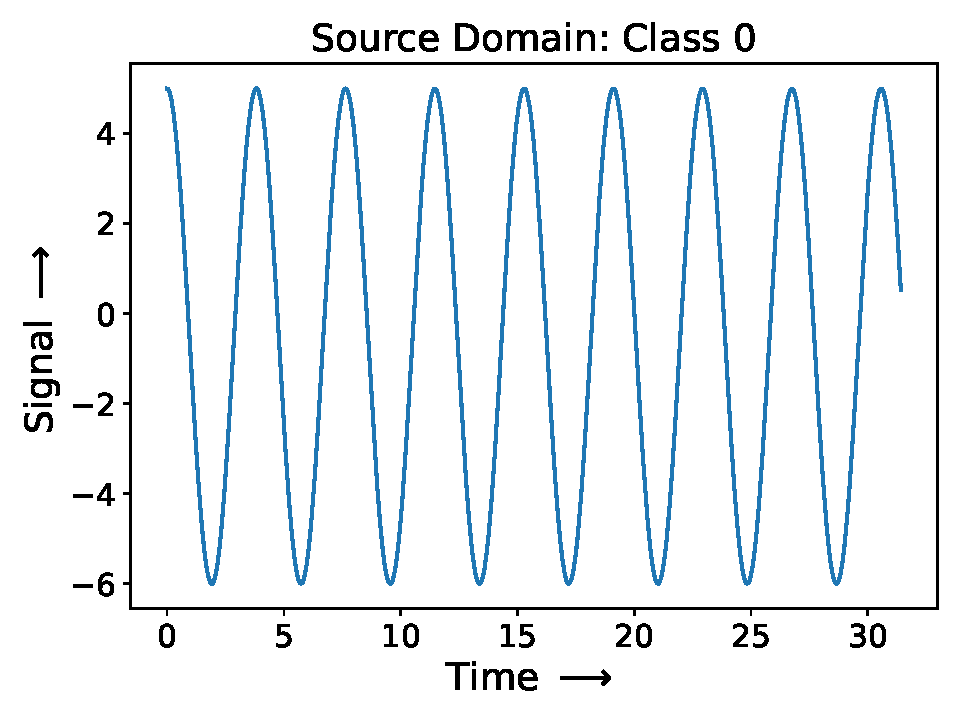
\includegraphics[width=.45\textwidth]{samples_domain_class_dummy_influence_noise/Source_Domain_Class_0_obs_1.pdf}
  \hspace{.3cm}
  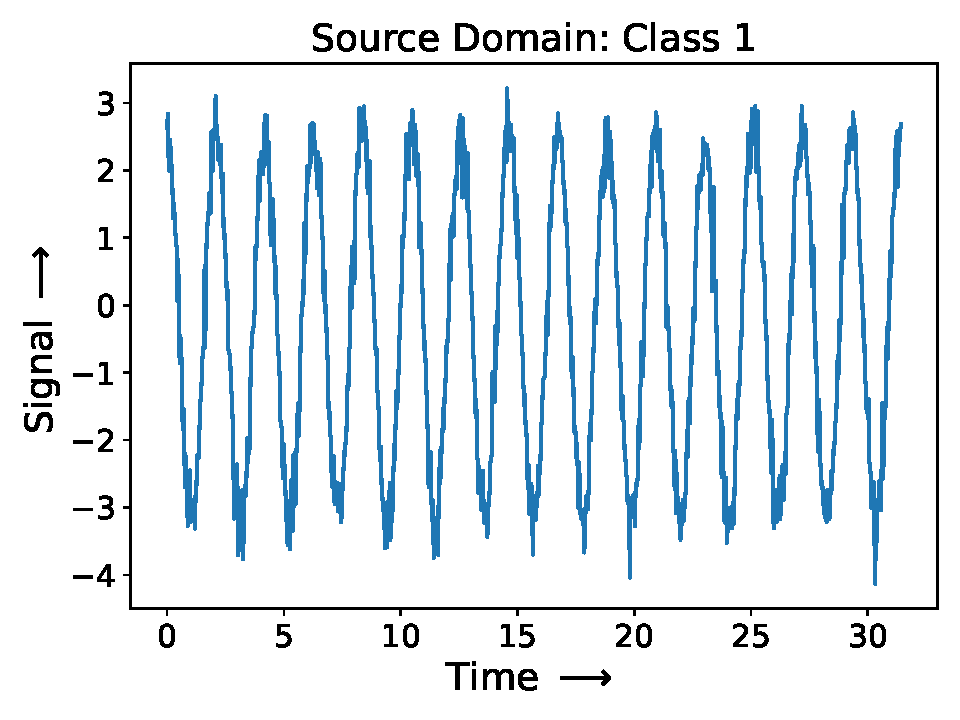
\includegraphics[width=.45\textwidth]{samples_domain_class_dummy_influence_noise/Source_Domain_Class_1_obs_1.pdf}

  \caption{Perturbation and noise during sampling process}
  \label{fig:samples_domain_class_dummy_influence_noise}
\end{figure}


\section{Dataset: Ball Screw Drive}
Testing the developed PHM methods on a real-world machine dataset is essential to make statements about the method's utility and applicability in the industry. In the following, the data collection from a milling machine is described in detail. Milling machines are common in the industry and contain several BSDs and LGSs, which suffer from continuous degradation. A continuous evaluation of the degradation state and replacement of these components is necessary. Due the industrial relevance of PHM for BSDs and LGSs, a corresponding dataset was recorded on a milling machine to evaluate the developed approaches.

\subsection{Experimental Setup}
Data from a DMG DMC 55H duoblock milling machine of the manufacturer DMG Mori was recorded. The machine tool’s spindle and housing, as well as the machine tool table, rotatory axes, peripherals, the cladding and the machine tool's housing were removed. The TNC control iTNC530 HSCI from Heidenhain GmbH was used. Fig. \ref{fig:experimental_setup} shows the experimental setup. The investigation focuses on the moving hanger assembly of the machine tool. The machine tool can be moved in the three spatial directions. The dataset just includes data from machine tool movements along the x-axis. For this reason, just the single threaded shaft of the BSD and the two LGSs, which are responsible for movements along the x-axis, are supervised.

\begin{figure}[H]
  \centering
  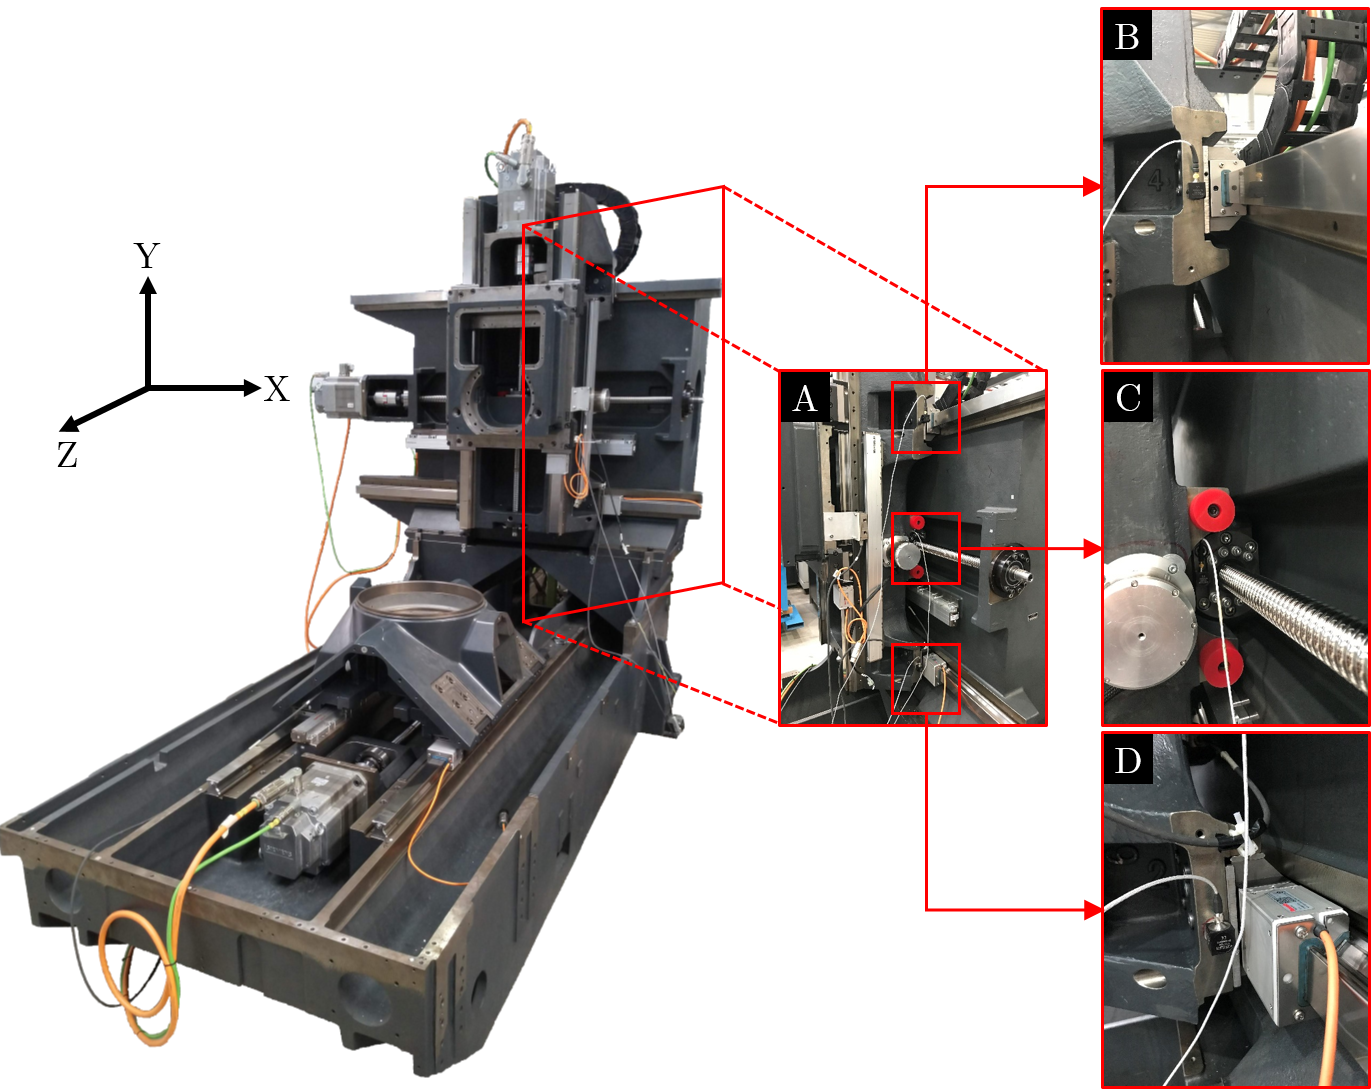
\includegraphics[width=0.9\textwidth]{experimental_setup}
  \caption {Experimental setup: s side-view of the machine, B: upper LGS, C: threaded shaft of BSD, C: lower LGS}
  \label{fig:experimental_setup}
\end{figure}

\subsection{Sensors}
The signals included in the dataset come from three different sources of measurement: acceleration sensors and internal control data accessed via TNC Scope and TNC Opt. The recordings of the three different sources were triggered by different software programs which were synchronized by a python script. Minor time delays between the signals could not be eliminated completely. Three triaxial Kistler 8762A10 piezo-eletric accelerometers were placed on different locations of the machine, recording accelerations in x,y,z-directions. The positions are specified in fig. \ref{fig:experimental_setup}. Accelerometers are placed at the upper LGS (sub-figure B), the BSD nut (sub-figure C) and the lower LGS (sub-figure D). The software tool TNC Scope was used to access the internal contol data of the machine. TNC Opt is a software tool, which is intended for controller optimization. During the experiments it was used to access those control data channels, which differ from those of TNC Scope.

\subsection{Definition of Degradation States}
Preload classes were defined, which specify the preload loss in the BSDs and LGSs. Besides that, in some of the BSDs pitting damages were observed. The degradation of BSDs and LGSs is defined by an ID containing one letter and two digits. The letter indicates the damage types: no pitting (C) or pitting (P). The first digit specifies the preload class and the second digit the observation. The preload loss was separated in three distinct classes. The assignment of the recorded samples to one of those classes is based on the measured preload forces (N) in the components. Low preload forces are the result of a high preload loss, which indicates a strong component degradation. This leads to a lower machine precision and a higher risk of machine failure. Preload class C3 is labelled as “healthy”, C2 as "slightly degraded" and C1 as "strongly degraded". Two sets of BSDs and one set of LGSs, each of them including all corresponding health condition classes, are part of the dataset. The observation digit helps to separate those equally degraded BSDs from the different sets. In total, ten recordings were made of all 24 combinations of differently degraded and observed BSDs and LGSs. The preload forces corresponding to the different health condition classes are specified differently for the observations. Table \ref {tab:BSDs_states} and table \ref {tab:LGSs_states} specify all BSDs and LGSs and their corresponding health condition classes. As described before the ID, containing one digit and two numbers, specifies the health condition of the BSDs and LGSs. The component name identifies the exact component used in the experimental setup during the recording. The experimental setup includes two LGSs, each consisting of two counterparts, and one BSD threaded shaft. Therefore, each BSD ID maps to one and each LGS ID to four components. The different combinations of LGSs and BSDs health condition classes during the recordings are shown in the table \ref{tab:recorded_combinations_of_LGS_and_BSD_health_conditions}.


\begin{center}
\begin{longtable}{c c c} 
\toprule
 ID & Component & Preload in N \\ [0.5ex] 
\midrule
 P1 & 721-14448-6-G6 & 2 070 \\ 
 P2 & 721-14448-4-G4 & 2 160 \\ 
 C11 & 721-14448-3-G3 & 950 \\ 
 C12 & 721-95859-4 & 845 \\ 
 C21  & 721-14448-1-G1 & 1 450 \\ [1ex] 
 C22  & 721-95859-2 & 1 293 \\ [1ex] 
 C31  & 721-14448-2-G2 & 2 390 \\ [1ex] 
 C32  & 721-95859-3 & 2 328 \\ [1ex] 
\bottomrule
\caption {BSDs health condition states}
\label {tab:BSDs_states}
\end{longtable}
\end{center}

\begin{center}
\begin{longtable}{c c c} 
\toprule
 ID & Component & Preload in N \\ [0.5ex] 
\midrule
 C1 & C1 & 4 060 \\ 
    & C2 & 4 430 \\ 
    & C3 & 4 430 \\
    & F1 & 3 880 \\ 
\midrule
 C2 & B1 & 8 860 \\ 
    & B2 & 9 700 \\ [1ex] 
    & B3 & 9 070 \\ [1ex]
    & E1 & 8 230 \\ [1ex]
\midrule
 C3 & A9 & 13 470 \\ 
    & A10 & 14 530 \\ [1ex] 
    & A11 & 12 840 \\ [1ex]
    & D3 & 12 840 \\ [1ex]
\bottomrule
\caption {LGSs health condition states}
\label {tab:LGSs_states}
\end{longtable}
\end{center}

\begin{comment}
\begin{center}
\begin{longtable}{c c c c c c c c c c} 
\toprule
%\multicolumn{10}{c}{BSD}
&&&&BSD&&&&
\cmidrule(lr){3-11}
  & & C31 & C21 & C11 & P1 & C22 & C12 & C32 & P2  \\ [0.5ex] 
\cmidrule(lr){3-11}
                          & C1 & 1 & 2 & 3 & 4 & 5 & 6 & 7 & 9 \\ 
LGS                       & C2 & 10 & 11 & 12 & 13 & 14 & 15 & 16 & 18  \\ 
                          & C3 & 19 & 20 & 21 & 22 & 23 & 24 & 25 & 27  \\
\bottomrule
\caption {Combinations of LGS and BSD health condition states}
\label {tab:recorded_combinations_of_LGS_and_BSD_health_conditions}
\end{longtable}
\end{center}
\end{comment}






\begin{center}
\begin{longtable}{c c c c c c c c c c} 
\toprule
  &  &    &     &     &     \multicolumn{2}{c}{BSD}     &     &     &    \\ 
  &  & C31 & C21 & C11 & P1  & C22 & C12 & C32 & P2 \\ 
\midrule
     & \multicolumn{1}{c|}{C1} & 1 & 2 & 3 & 4 & 5 & 6 & 7 & 9 \\ 
 LGS & \multicolumn{1}{c|}{C2}& 10 & 11 & 12 & 13 & 14 & 15 & 16 & 18 \\  
     & \multicolumn{1}{c|}{C3} & 19 & 20 & 21 & 22 & 23 & 24 & 25 & 27 \\ 
\bottomrule
\caption {Combinations of LGS and BSD health condition states}
\label {tab:recorded_combinations_of_LGS_and_BSD_health_conditions}
\end{longtable}
\end{center}


\subsection{Recording of Dataset}
For the sake of reproducibility, the experiments are executed with a defined test cycle, which is defined in fig. \ref{fig:test_cycle}. Machine data is collected during constant speed, direction change and sweep excitement along the machine tools X-axis. During the constant speed excitement, the machine tools are moved back and forth along the whole axis ($\Delta x$ = 600mm). During the direction change excitation, the movement of the machine tools is restricted to a small part of the axis ($\Delta x$ = 1mm) and the directions are changed with a high frequency. In the sweep excitement, the motor receives a target speed in the form of a sine sweep. Before recording data, the machine is warmed up for 60min with a constant speed excitement to create equivalent circumstances for all runs.

\begin{figure}[H]
  \centering
  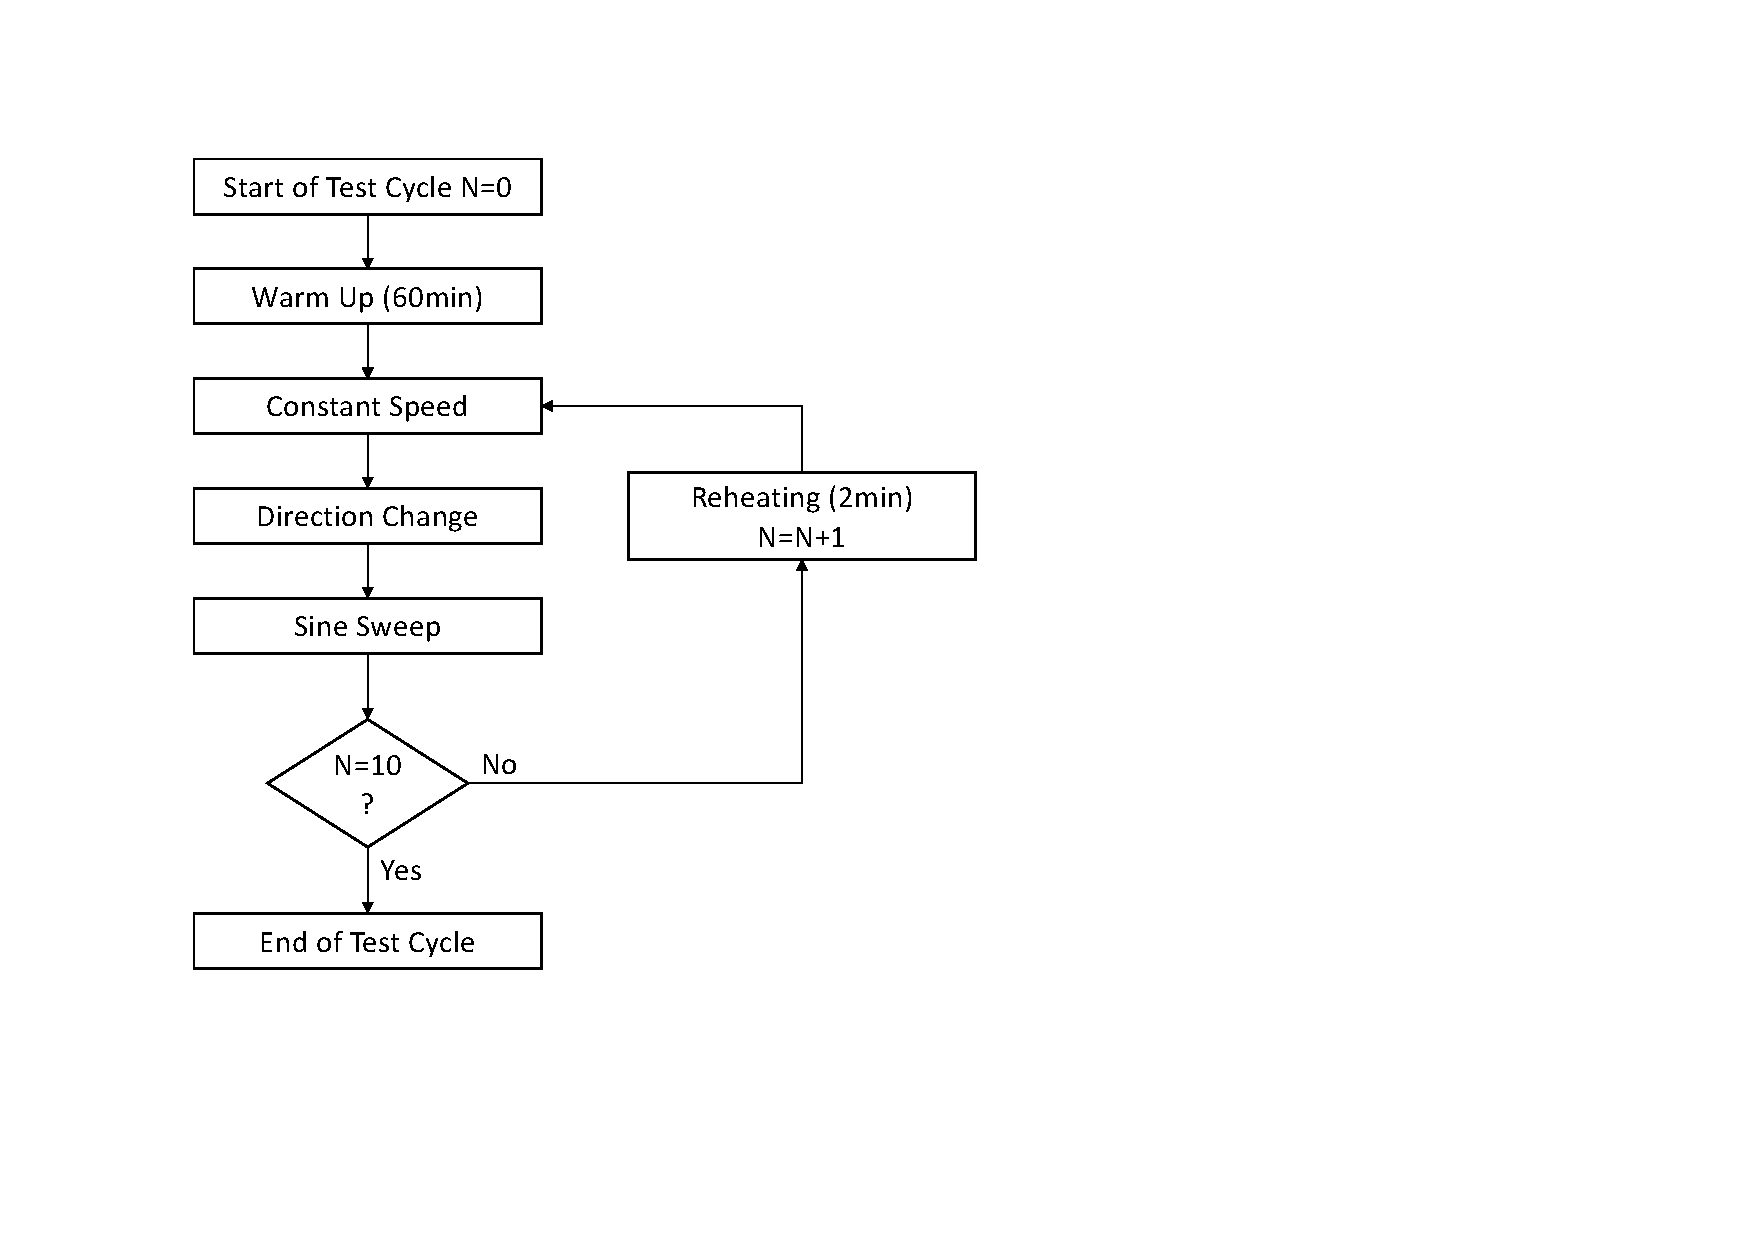
\includegraphics[width=0.7\textwidth]{test_cycle.pdf}
  \caption {Test cycle for data recording}
  \label{fig:test_cycle}
\end{figure}

In total 49 different signals are recorded from the previously described three data sources. The signals are specified in more detail in table. \ref{tab:description_of_the_49_recorded_features}. All feature names starting with "C" correspond to the constant speed , "D" to the direction change and "S" to the sweep excitement.

\begin{center}
\begin{longtable}{c c c c} 
 \toprule
 Signal & Sensor & Frequency & Samples \\ [0.5ex] 
 \midrule
 C:s ist/X & TNC Scope & 10 kHz & 75000 \\ 

 C:s soll/X & TNC Scope & 10 kHz & 75000 \\ 

 C:s diff/X & TNC Scope & 10 kHz & 75000 \\ 

 C:v (n ist)/X & TNC Scope & 10 kHz & 75000 \\ 

 C:v (n soll)/X& TNC Scope & 10 kHz & 75000 \\ 

 C:P mech./X & TNC Scope & 10 kHz & 75000 \\ 

 C:Pos. Diff./X & TNC Scope & 10 kHz & 75000 \\ 

 C:I ist/X & TNC Scope & 10 kHz & 75000 \\ 

 C:I soll/X & TNC Scope & 10 kHz & 75000 \\ 

 C:x bottom & Acc & 10 kHz & 75000 \\ 

 C:y bottom & Acc & 10 kHz & 75000 \\ 

 C:z bottom & Acc & 10 kHz & 75000 \\ 

 C:x nut & Acc & 10 kHz & 75000 \\ 

 C:y nut & Acc & 10 kHz & 75000 \\ 

 C:z nut & Acc & 10 kHz & 75000 \\ 

 C:x top & Acc & 10 kHz & 75000 \\ 

 C:y top & Acc & 10 kHz & 75000 \\ 

 C:z top & Acc & 10 kHz & 75000 \\ 

 D:s ist/X & TNC Scope & 10 kHz & 75000 \\

 D:s soll/X & TNC Scope & 10 kHz & 75000 \\ 

 D:s diff/X & TNC Scope & 10 kHz & 75000 \\ 

 D:v (n ist)/X & TNC Scope & 10 kHz & 75000 \\ 

 D:v (n soll)/X & TNC Scope & 10 kHz & 75000 \\ 

 D:P mech./X & TNC Scope & 10 kHz & 75000 \\ 
 
 D:Pos. Diff./X & TNC Scope & 10 kHz & 75000 \\ 

 D:I ist/X & TNC Scope & 10 kHz & 75000 \\ 

 D:I soll/X & TNC Scope & 10 kHz & 75000 \\ 

 D:x bottom & Acc & 10 kHz & 75000 \\ 

 D:y bottom & Acc & 10 kHz & 75000 \\ 

 D:z bottom & Acc & 10 kHz & 75000 \\ 

 D:x nut & Acc & 10 kHz & 75000 \\ 

 D:y nut & Acc & 10 kHz & 75000 \\ 

 D:z nut & Acc & 10 kHz & 75000 \\ 

 D:x top & Acc & 10 kHz & 75000 \\

 D:y top & Acc & 10 kHz & 75000 \\ 

 D:z top & Acc & 10 kHz & 75000 \\ 

 S:x bottom & Acc & 10 kHz & 153601 \\ 

 S:y bottom & Acc & 10 kHz & 153601 \\ 

 S:z bottom & Acc & 10 kHz & 153601 \\ 

 S:x nut & Acc & 10 kHz & 153601 \\ 

 S:y nut & Acc & 10 kHz & 153601 \\ 

 S:z nut & Acc & 10 kHz & 153601 \\ 

 S:x top & Acc & 10 kHz & 153601 \\ 

 S:y top & Acc & 10 kHz & 153601 \\ 
 
 S:z top & Acc & 10 kHz & 153601 \\ 
 
 S:Nominal rotational speed & TNC opt & 1 kHz & 16384 \\
 
 S:Actual rotational speed & TNC opt & 1 kHz & 16384 \\ 
 
 S:Actual position of the position encoder(dy/dt) & TNC opt & 1 kHz & 16384 \\ 
 S:Actual position of the motor encoder(dy/dt)  & TNC opt & 1 kHz & 16384  \\ [1ex] 
 \bottomrule
\caption {Description of recorded signals}
\label {tab:description_of_the_49_recorded_features}
\end{longtable}
\end{center}


\subsection{Definition PHM Task on the Ball Screw Drive Dataset}
In this thesis a PHM model for binary classification of BSD health condition classes is developed. To create a binary classification problem C2 and C3 are combined in a "healthy" and C1 and P1 a "degraded" class. A domain shift is generated by combining all samples recorded with BSDs from observation 1 in the source and from observation 2 in the target domain. Since the BSD preload classes are defined differently for both observations (see table \ref{tab:BSDs_states}) a domain shift is guaranteed. Besides that, marginal differences in the production and installation of the BSDs can lead to domain shifts. Independent of the LGS abrasion level, the PHM model should be able to predict the BSD health condition class accurately. The experiments of Li et al. \cite{Li2018} showed, that the lifetime of BSDs is shorter than that of LGSs. This means, that BSDs need to be replaced in shorter internals than LGSs. Throughout the lifetime of an industrial machine, it is very common that BSDs and LGSs with different levels of degradation are combined. Often times the dataset for training a PHM model is extracted from an experimental setup including a specific set of BSDs and LGSs. Later the PHM model should work with a high accuracy on data recorded from a different set of BSDs and LGSs. For these reasons, the defined task for this thesis is quite realistic.

\section{Methods}\label{chapter:introduction}
In the following, the model architecture as well as the applied training concept, which are used in this thesis, are presented. The models applied on the dummy and real-world dataset do all have the same architecture. The presented training concept applies to all models used in the real world dataset. During the primary evaluation of different approaches on the dummy dataset, different training techniques were implemented. In the chapters of section \ref{sec:results_dummy_dataset} the deviations from the now presented training strategies are clarified.

\subsection{Model}
\label{sec:model}
The model used during the experiments consists of a 1D CNN and a subsequent classifier. The CNN extracts expressive features which are later used by the classifier to predict the health condition class of the BSDs. A more detailed visualization of the architecture is shown in fig. \ref{fig:proposed_model}. The CNN consists of three convolutional layers. With increasing network depth the spatial dimension of the feature map is decreased and its channel size increased. This helps to extract more global features in shallow and more specific and local features in deeper layers. The exact parameters of the convolutional layers are specified in table \ref{tab:parameter_conv} 

\begin{longtable}{c c c c} 
\toprule
Parameter & Conv 1 & Conv 2 & Conv 3 \\
\midrule
kernel size & 100 & 10 & 5 \\

padding size & 0 & 1 & 1 \\

stride & 1 & 1 & 1 \\
\bottomrule
\caption {Parameter in convolutional layer}
\label {tab:parameter_conv}
\end{longtable}

Pooling layers are included after the convolutional layers to reduce the spatial dimension of the feature maps. Reducing the model complexity prevents problems like overfitting and exploding gradients. Applying batch normalization after convolutional layers fixes the means and variances of the layer's input for each batch. This helps to make the training faster and more stable. After iteratively applying these three types of layers the output of the CNN is flattened and normalized to a 1D vector. This vector is fed in the subsequent classifier. The latent feature space dimensions of the classifier are reduced constantly. The two neurons in the output layer of the neural network represent the prediction probability for the two defined BSD health condition classes.


\begin{figure}[H]
  \centering
  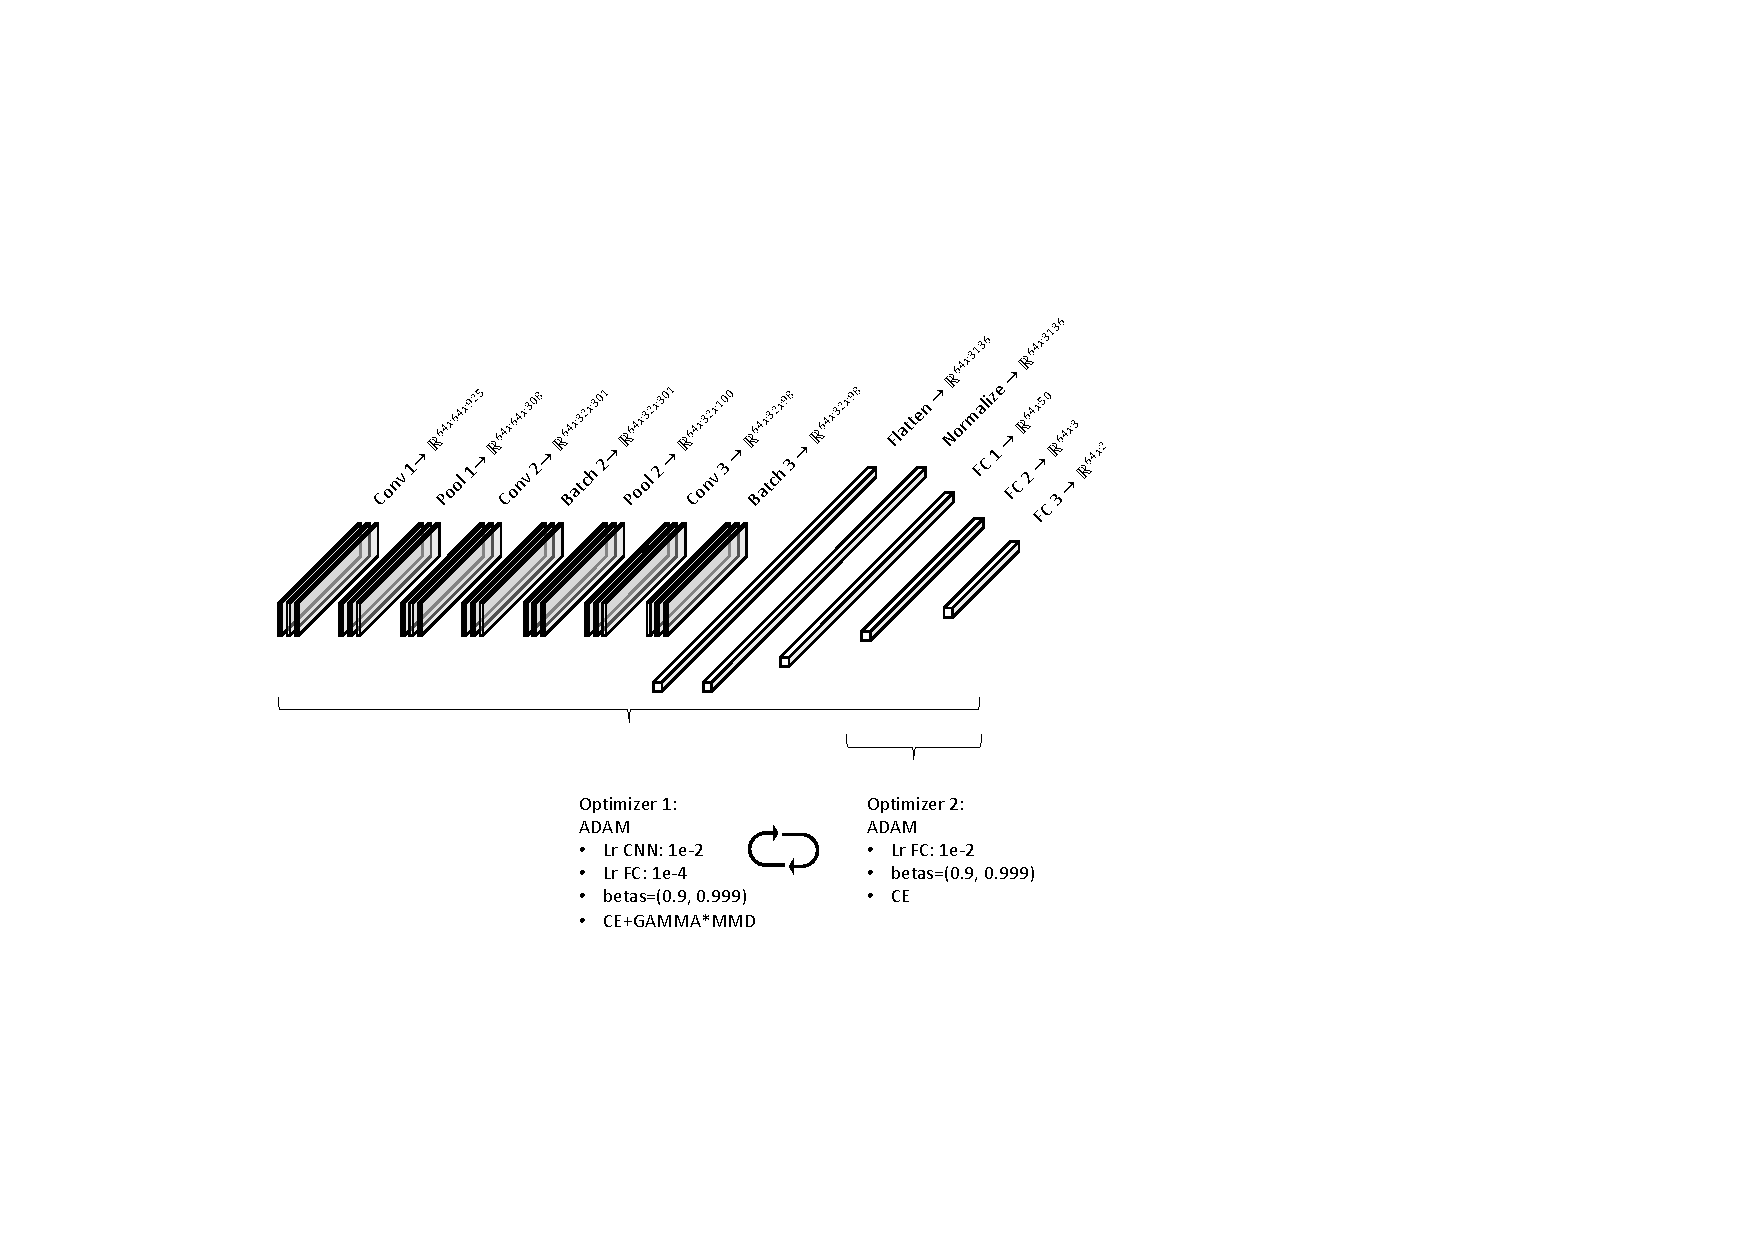
\includegraphics[width=1\textwidth]{proposed_model.pdf}
  \caption {Proposed model} \label{fig:proposed_model}
\end{figure}


\subsection{Proposed Training with MMD- and CE-Loss} \label{sec:Proposed_training}

Firstly, the data used for the training is pre-processed. The dataloader separates the data in shorter sequences of length 1024. These windows, which can include several of the recorded 49 signals, are fed as single samples to the model. The sequenced signals are cleaned from Nan values. The signals contained in one sequence are synchronized. Separate source and target domain dataloader were created, which split the corresponding datasets in four different parts: MMD-Training (40\%), CE-Training (20\%), Validation (20\%) and Testing (20\%). Other pre-processing steps, like wavelet transforms, can easily be added to the dataloader. The repetitive training of the model is visualized in fig. \ref{fig:Training_Process_MMD}. A weighted average of a source CE and MMD-loss is applied to optimize the proposed deep learning-based domain adaptation model. The MMD-loss estimates the domain discrepancy in several latent feature maps. The MMD-loss facilitates the extraction of domain invariant features. The domain discrepancy is measured as squared distance between the distribution kernel embeddings in the reproducing kernel Hilbert space (RKHS). The kernel choice is of great importance for the performance of the MMD-loss. For this reason, several RBF kernels with bandwidth parameters 1, 2, 4, 8, 16 were combined to profit from their individual strength. The source and target samples are randomly coupled up and processed by the MMD-loss. The class of these samples is not considered in the MMD-loss. Therefore, the MMD-loss minimizes the domain discrepancy between source and target domain of different and equal classes. The MMD is applied in several layers of the CNN and classifier. The source CE-loss is applied in the last fully connected layer and optimizes the model to increase the classification accuracy on the source domain. Fig. \ref{fig:MMD_Loss_and_CE_loss} symbolically shows how the MMD and the source CE-loss is applied in different layers of the model.



\begin{figure}[H]
  \centering
  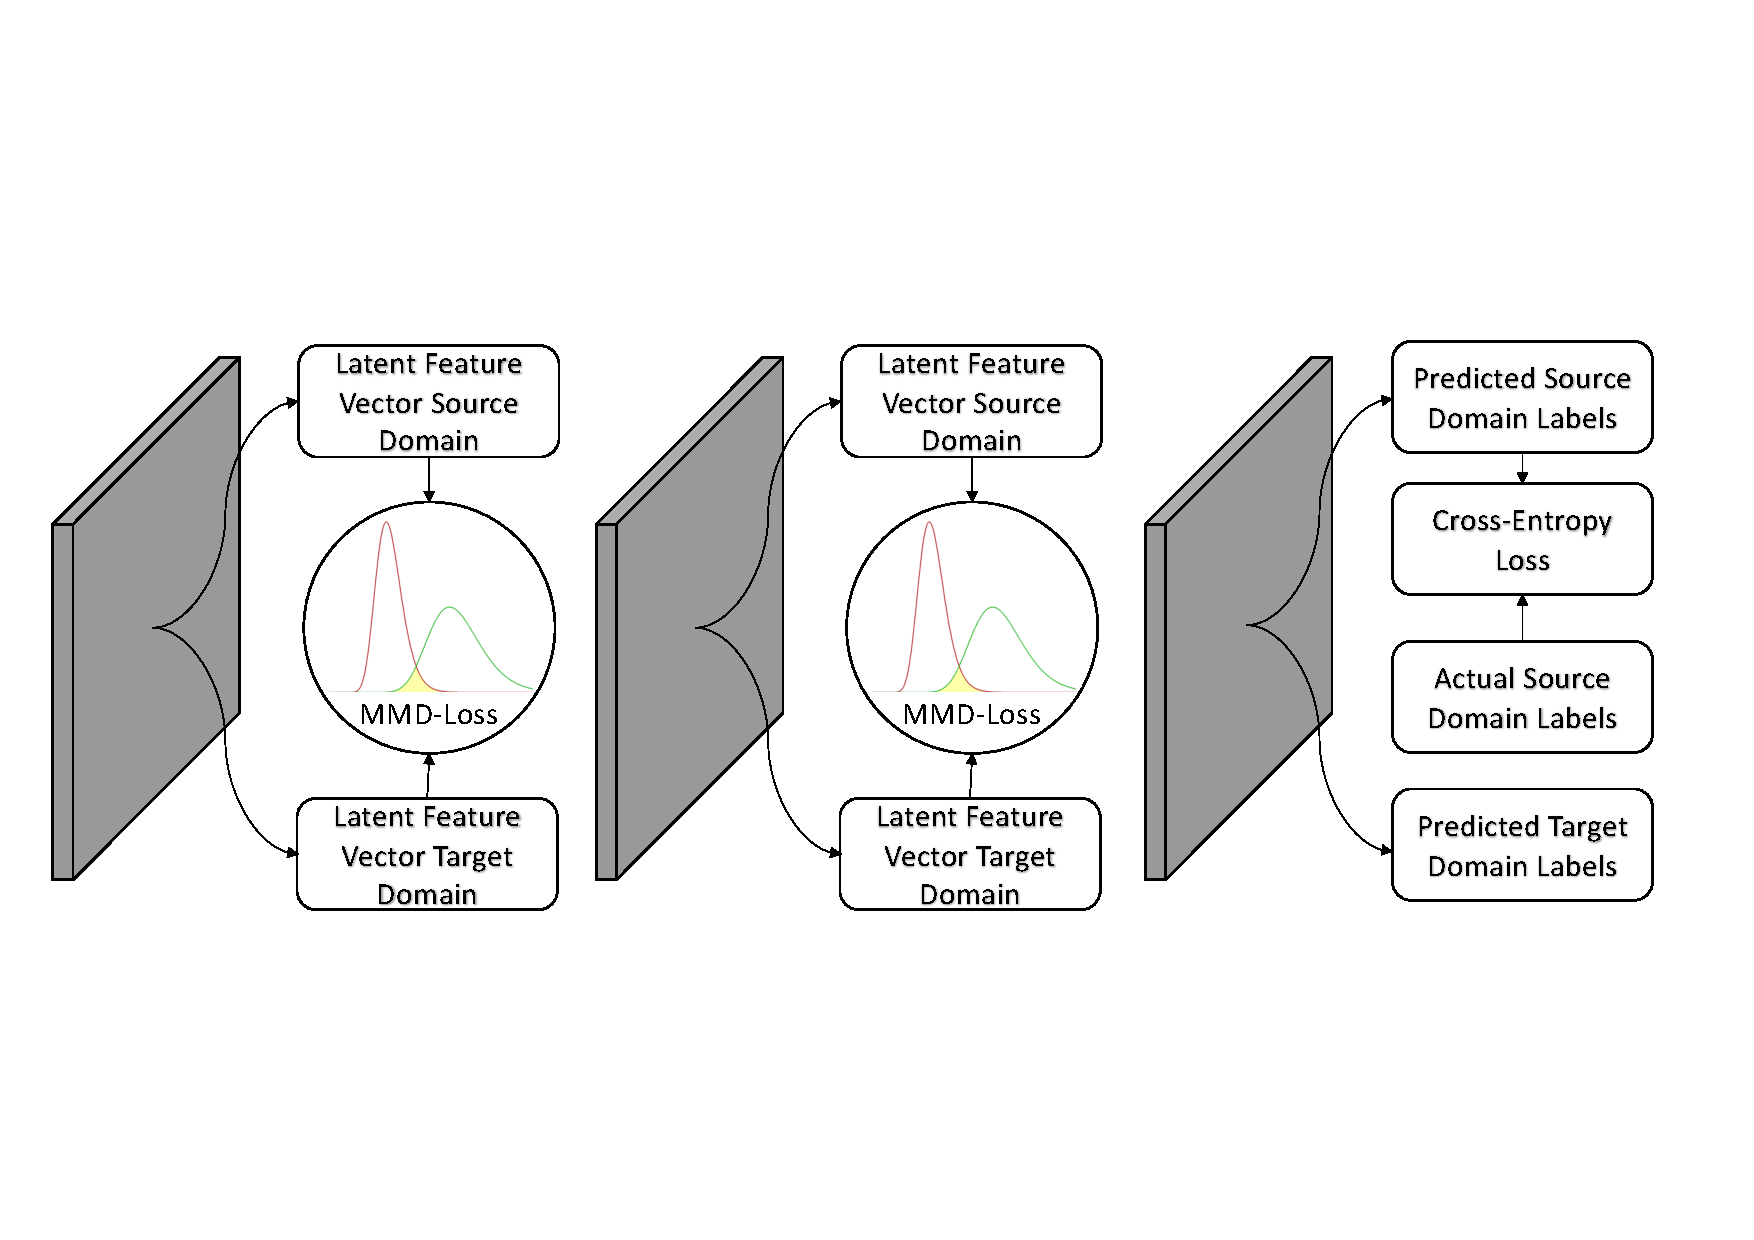
\includegraphics[width=1\textwidth]{MMD_loss_visualization.pdf}
  \caption {CE- and MMD-loss in neural networks} \label{fig:MMD_Loss_and_CE_loss}
\end{figure}
 
A total loss must be specified by defining a weighted average between the MMD and source CE-loss. The weighting factor GAMMA is a hyperparameter, which need to be defined beforehand. The total loss is defined as following:

\begin{equation}
    \mbox{Total Loss} = \mbox{Source CE-Loss} + \mbox{GAMMA} \cdot \mbox{MMD-Loss}
\end{equation}.

The model training is separated in two phases. In a first phase, the total loss is used to optimize the whole network. An ADAM optimizer is used with different learning rates for the layers Conv1 - FC1 (lr=1e-2) and FC2 - FC3 (lr=1e-4). In a second phase, just the CE-loss is applied to optimize the final two fully connected layers. Again an ADAM optimizer with a learning rare of 1e-2 is used. In both optmization steps the beta values are 0.9 and 0.999. Two-thirds of the training data is used in the first and one-third in the second train phase. The application of two different optimizer is visualized in fig. \ref{fig:proposed_model}. In general, the training is repeated until the maximum number of epochs is reached. After the training is completed, the model can be used to predict the BSD health condition state of unseen target domain samples. 

\begin{figure}[H]
  \centering
  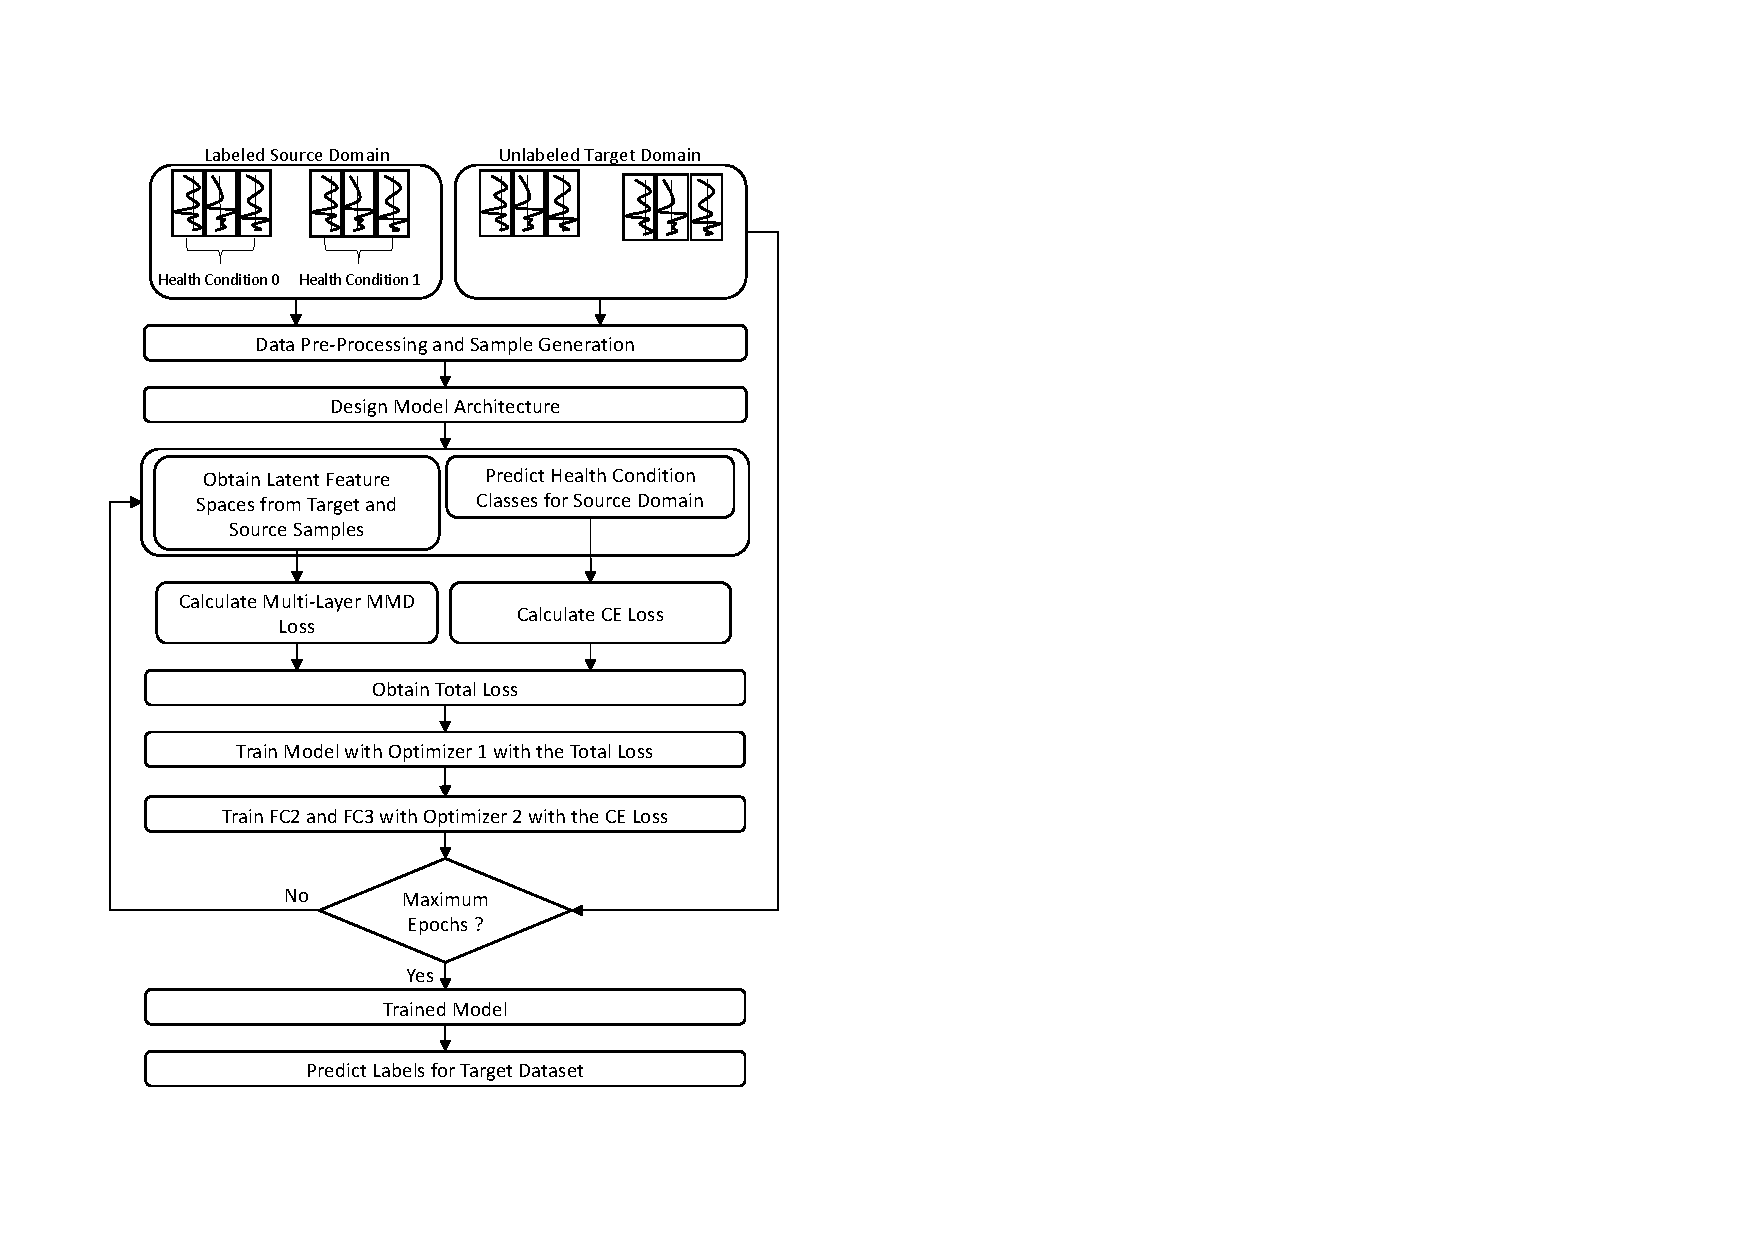
\includegraphics[width=0.8\textwidth]{training_process_mmd.pdf}
  \caption {Model training} \label{fig:Training_Process_MMD}
\end{figure}

